\label{fs-formalism}

\subsection{Reference streaming model}

\begin{definition}{Reference stream processing system}
is a tuple of $(\Gamma,D)$, where $\Gamma$ is a set of all possible data flow elements, and $D\subseteq{\Gamma\times\Gamma}$ is a binary relation on it. Pair $(x,y)\in{D}$ if $y$ can be generated from $x$ within physical graph. We assume that all user-defined operations are pure.
\end{definition}

Within our model, one can define streaming system using only data flow elements and business logic. However, without the notion of time, we cannot observe any processing progress. Let $\tau\in{\mathbb{N}}$ be an exact global discrete time. Let $a_\tau\in{\Gamma}$ be the element, which enters at the time $\tau$, and $b_\tau\in{2^\Gamma}$ be the elements, which leave at the time $\tau$. Let $A_{\tau}=\{a_i\}^{\tau}_{i=1}$ be a set of all input elements by the time $\tau$ and ${B}_\tau=\bigcup\limits_{i=1}^{\tau}{b_i}$ be a set of all output elements.

\begin{definition}{A reference working set}
$\widehat{W}_\tau\subseteq{\Gamma}$ at the time $\tau$ is the set of elements, which are currently in the reference system:

$\widehat{W}_0=\emptyset$:

$\widehat{W}_{\tau+1}=\begin{sqcases}
\widehat{W}_{\tau}\cup{a_{\tau+1}}, & \text{or}\\
\widehat{W}_{\tau}\setminus{b_{\tau+1}}, & \text{or}\\
\widehat{W}_{\tau}\setminus{X}\cup{Y}, \forall{x\in{X}\exists{y\in{Y}}}:(x,y)\in{D} & \text{}.
\end{sqcases}$

\end{definition}

We can imagine a stream processing system as a pool, where some elements are poured in and others are poured out. Inside a pool, each element can be substituted by the other element, which can be substituted as well, and so on. Only survived elements are poured out from the pool.

\begin{definition}{System state}
$S_\tau$ at the time $\tau$ is $\widehat{W}_\tau^{\infty}$ if $A_{\infty}=\{a_i\}^{\tau}_{i=1}$.
\end{definition}

\begin{definition}{Nullification time}
of an input element $a_\tau$ is the first moment of time when all elements that depends on $a_\tau$ are in state or released from the system, $\theta_{a_\tau}=inf(\hat{\tau}>\tau|W_{\hat{\tau}}\setminus{S_{\hat{\tau}}}\cap{Cl(D)(a_\tau)=\emptyset})$, where $Cl(D)$ is a transitive closure of the relation $D$.
\end{definition}

State is a set of all data flow elements that stay in the system if we block input and wait for an infinite time. Technically, states in existing stream processing systems are not data flow elements, but as it was mentioned above, they can be presented in such a way using drifting state model. The main purpose of the state is to accumulate the information about input items. Data flow elements cannot be in $W\setminus{S}$ for an infinite time by the definition of state. Hence, for each input element $a_\tau$, there is a nullification time $\theta_{a_\tau}$, thereafter all elements, which depend on $a_\tau$, are in the system state. Since the nullification time, the input element can affect output elements only through the state.

Since we cannot observe internal transitions directly, it is convenient to limit global time domain only to moments of output events.

\begin{definition}{Time quantization}
$\tau(t)$ is monotonic mapping from time domain restricted to only output events to global discrete time $\tau$, $\forall{t}\exists{b_{\tau(t)}}$.
\end{definition}

\begin{definition}{Probability of output element in a reference system}
$p(b_{t+1}|A_{t+1}, B_t)$ is a probability to observe output element $b$ at the time $t+1$ considering all previous input and output elements. For all output elements from the reference working set, such probability is positive,\\
$\forall{b_{t+1}:\exists{\widehat{W}_{t+1}=\widehat{W}_{t}\setminus{b_{t+1}}}} \Rightarrow p(b_{t+1}|A_{t+1}, B_t) > 0$.
\end{definition}

In classical distributed system model proposed in~\cite{Chandy:1985:DSD:214451.214456}, a distributed system is defined as a graph of processes, which can be connected to each other via channels. Each process can generate {\em events} and send them to other processes through the channels. Global system state in this model contains processes states and channel states, e.g., elements, which are in-flight at the moment. Distributed asynchronous processing is simulated using permutations of events. 

In terms of Chandy-Lamport model, the global state of our streaming model contains only channel states, while events are input elements, output elements, and user-defined transformations. We model the asynchronous nature of distributed processing via global discrete time, that does not determine a priori order of transformations. There is only a probability to observe some specified output element, even in the reference system. However, our model has a significant distinction: it is assumed that end-user is external to the system, i.e., a user is able to observe output elements, but not the system states. Hence, as we show further, the notion of {\em consistency} in this case should also be defined in terms of output elements.  

\subsection{Streaming model with failures}

Unfortunately, the reference stream processing system is just an abstract concept, because it does not capture probable failures of network and computational units. Failure can be expressed as a loss of the working set or its part. There is a need to extend the reference model by recovering mechanism that allows a system to transparently pass through the failures.

{\bf Snapshot = set!}

\begin{definition}{Stream processing system}
is a tuple of\\
$(\Gamma,D,P,F)$. $\Gamma$ and $D$ are the same as in the reference system. Snapshot $P$ is an information about system execution that is available even in case of a system failure. At time $\tau$ snapshot contains information $P_\tau$. Recovery function $F(A^{p}_\tau,P_\tau)$ provides logic for recovering of working set in case of system failures based on some set of input elements and a snapshot.
\end{definition}

\begin{definition}{Working set}
$W_\tau\subseteq{\Gamma}$ at the time $\tau$ is the set of elements, which are currently in the system:

$W_0=\emptyset$:

$W_{\tau+1}=\begin{sqcases}
W_{\tau}\cup{a_{\tau+1}}, & \text{or}\\
W_{\tau}\setminus{b_{\tau+1}}, & \text{or}\\
W_{\tau}\setminus{X}\cup{Y}, \forall{x\in{X}\exists{y\in{Y}}}:(x,y)\in{D} & \text{or}\\
F(A^{p}_\tau,P_\tau), A^{p}_\tau\subseteq{A_\tau} & \text{}.
\end{sqcases}$

\end{definition}

{\bf Working set captures the same transitions as the reference working set, but it also has a {\em recovery transition}.}

\begin{definition}{Probability of output element}
$\widetilde{p}(b_{t+1}|A_{t+1}, B_t)$ is a probability to observe output element $b$ at the time $t+1$ considering all previous input and output elements.
\end{definition}

\subsection{Consistency guarantees}

The reference system concept allows us to express the notion of valid execution in terms of correspondence between input and output elements. In most real cases, input and output elements are the only data that can be observed by end-user. In real distributed stream processing systems, failures and recoveries can corrupt the output, despite the fact, that in terms of a naive definition of delivery guarantees, all elements are processed exactly one time. Let us demonstrate it by an example. Assume that execution graph consists of a single operation $V^{i+1}=a_\tau(1+V^{i}),V^{0}=0,V\in{S}$ and $\forall{t},b_t=V$. In case of failure and recovery, the consistency of subsequent results depends not only on further input elements but on the restored $V$ as well. If a system recovers $V$ incorrectly after a failure, the results may become invalid. For instance, if $V=0$ after recovery, but before failure it was equal to some value $q\neq{0}$, end-user will receive unexpected output, even if each input element $a_\tau$ is processed exactly once. This example is demonstrated in Figure~\ref{state-inconsistency}. 

\begin{figure}[htbp]
  \centering
  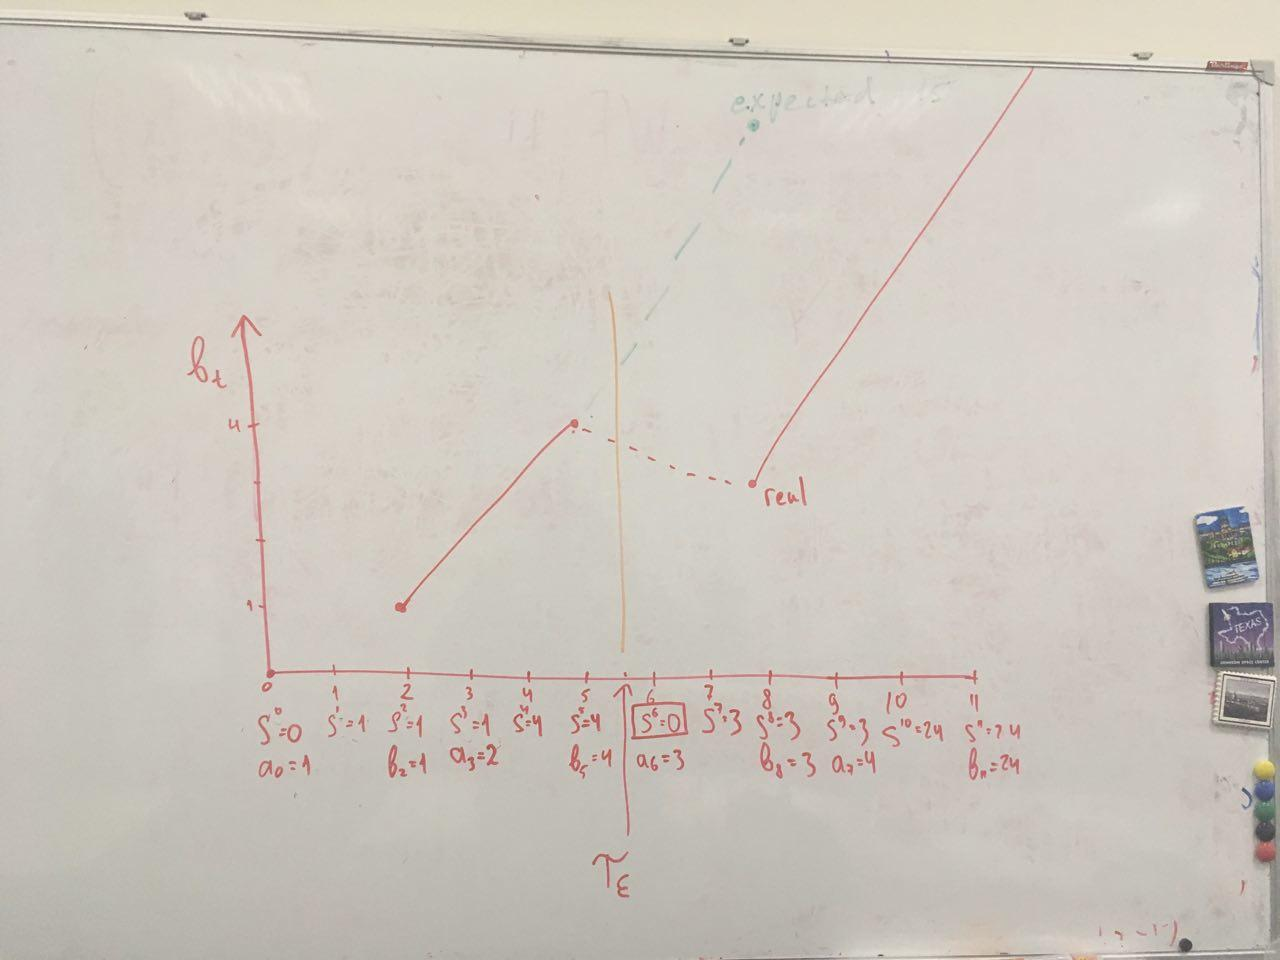
\includegraphics[width=0.48\textwidth]{pics/state-inconsistency}
  \caption{Inconsistency of results after incorrect recovery}
  \label {state-inconsistency}
\end{figure}

\begin{definition}{System provides for exactly once}
if it is possible to obtain each output element $b_{t+1}$ in the reference stream processing system, i.e.,\\ 
$\forall{t} \forall{b_{t+1}}: \widetilde{p}(b_{t+1}|A_{t+1},B_t)>0 \Rightarrow p(b_{t+1}|A_{t+1},B_t)>0$.
\end{definition}

\begin{definition}{System provides for at most once}
if \\
$\exists{A^{0}_{t+1}\subseteq{A_{t+1}}}$ such that \\
$\forall{t} \forall{b_{t+1}}: \widetilde{p}(b_{t+1}|A_{t+1},B_t)>0 \Rightarrow p(b_{t+1}|A^{0}_{t+1},B_t)>0$.
\end{definition}

\begin{definition}{System provides for at least once}
if \\
$\exists{A^{*}_{t+1}\subseteq{2^{A_{t+1}}}}$ such that \\
$\forall{t} \forall{b_{t+1}}: \widetilde{p}(b_{t+1}|A_{t+1},B_t)>0 \Rightarrow p(b_{t+1}|A^{*}_{t+1},B_t)>0$.
\end{definition}

Exactly once states that observed results cannot be distinguished from one of the possible results produced by the reference system. At most once and at least once guarantees are the relaxations of exactly once. The results within these guarantees can be obtained in the reference system, but with the assumption, that input is not completely correct. At least once can be reproduced if the input contains duplicates. At most once can be achieved in the reference system if some input elements are missed. It is important to note, that regarding at most once guarantee we require an input element to be processed atomically with all its derivatives or not processed at all. To the best of our knowledge, no one real stream processing engine supports at most once guarantee, so we cannot verify the relevancy of this assumption. 

% странно
% погрепать only и посмотреть на порядок
% outputting -> releasing, sending out
Thus, we can relax system recovery mechanisms by possible input channel flaws. This trick allows us to represent invisible system details in clear for user terms.

We can proceed from the probability of output element to the probability of the working set through the formula of total probability:

$p(b_{t+1}|A_{t+1},B_t)=\\
\sum\limits_{W_{t+1}}p(W_{t+1}|A_{t+1},B_t)p(b_{t+1}|A_{t+1},B_t,W_{t+1})=\\
\sum\limits_{W_{t+1}}p(W_{t+1}|A_{t+1},B_t)p(b_{t+1}|W_{t+1})
$.

Hence, in order to preserve exactly once, system must preserve working set that is possible to observe in reference system, because $\forall{t} \forall{b_{t+1}} p(b_{t+1}|A_{t+1},B_t)>0$ only if $\forall{t} \exists{W_{t+1}}:p(W_{t+1}|A_{t+1},B_t)>0$.

\begin{definition}{Snapshotting mechanism $P,F$ is consistent}
if $\forall{t} \exists{A^{p}_t\subseteq{A_t}} : p(F(A^{p}_t,P_t)|A_{t+1},B_t)>0$.
\end{definition}

% MillWheel ensures that $F(\emptyset,P_t)=\widehat{W_t}$ using strong productions and deduplication.

\begin{definition}{State snapshot}
$P^{s}$ is a snapshot such that $\forall{t} P^{s}_t = S_{t_s},t_s \leq t$.
\end{definition}

A streaming system must provide for consistent state snapshotting mechanism in order to support exactly once processing by the definition. Further, we demonstrate the ways how it is done in state-of-the-art solutions, but before it, we formally show the basic motivation behind some of them. 

One of the main factors that affects a method of taking a snapshot is the amount of information that is included in the snapshot. An obvious idea is to maintain the whole $W$, like it is done in MillWheel. Some other industrial systems, like Flink and Storm, save only system state, that takes up less disk space in general. However, state snapshotting imposes additional restrictions on the snapshot structure and mechanism.

\begin{theorem}
\label{necessary_conditions}
The necessary conditions of consistent state snapshotting are:\\
1. $\forall{b_t}:P^{s}_t=S_t$\\
2. $\forall{t}\forall{a}\notin{A^{p}_t} : \theta_a \leq t$
\end{theorem}
\begin{sketch}
$ $\newline
1. Assume that $\exists{b_t}:P^{s}_t = S_{t_s}, t_s < t$. Let system fails at $\tau_f = \tau(t)+1$. Let $(a_{\tau(t_s)+1},y)\in{D}$ and $y\in{S_t}$. In this case, recovery function must reprocess $a_{\tau(t_s)+1}$ in order to achieve $W_t=F(A^{p}_t,S_{t_s})\supseteq{S_t}$ that is possible in the reference system. However, reprocessing of $a_{\tau(t_s)+1}$ can cause some output $ b_{t+1}\in{Cl(a_{\tau(t_s)+1})}$, such that $p(b_{t}|A_t,B_{t-1})=0$, because $B_{t-1}$ can already contain output elements that have been generated from element $a_{\tau(t_s)+1}$ before reprocessing. \\
2. Assume that $\exists{t} \exists{a} \notin{A^{p}_t}:\theta_{a}>t$. In this case, $Cl^{-1} \cap (W_t \setminus{S_t}) \neq \emptyset$. If system fails at time $\tau_f=\tau(t)+1$, elements $Cl^{-1} \cap (W_t \setminus{S_t})$ cannot be restored using $A^{p}_t$ and $P^{s}_t=S_t$, because restoring requires reprocessing of element $a$.
\end{sketch}

This theorem has a direct practical implication. If a system that uses state snapshots aims at providing for exactly once, it must output elements $b_t$ only if there exists a snapshot for time $t$. It means that the lower bound of latency in the worst case in such systems is the snapshotting period together with the duration of taking a snapshot. There is a trade-off between latency and the frequency of taking snapshots because too frequent snapshotting can cause high extra load, while rare snapshots lead to high latency.

\begin{definition}{System is deterministic}
if\\ 
$\forall{b_{t+1}},p(b_{t+1}|A_{t+1},B_t)=1$.
\end{definition}

The following theorem shows that for a deterministic system the first condition of a Theorem~\ref{necessary_conditions} can be relaxed. 

\begin{theorem}
\label{determinism}
If system is deterministic, state snapshot is extended with the last output element: $\forall{b_t}:P_t=P^{s}_t \cup b_t$, and $\forall{t}\forall{a}\notin{A^{p}_t} : \theta_a \leq t$, then system is able to provide exactly once.
\end{theorem}
\begin{sketch}
Assume that $\exists{b_t}:P_t = S_{t_s} \cup b_t, t_s < t$. Without loss of generality, assume that system fails at the time $\tau_f = \tau(t)+1$. The problem here is that if $(a_{\tau(t_s)+1},y)\in{D}$ and $y\in{S_t}$, recovery function must reprocess $a_{\tau(t_s)+1}$ in order to achieve $W_t=F(A^{p}_t,S_{t_s})\supseteq{S_t}$ that is possible in the reference system. However, reprocessing can cause inconsistent output as it is shown in Theorem~\ref{necessary_conditions}. The property of determinism guarantees that in case of reprocessing output elements will be the same and released in the same order. Having last outputted before the failure element $b_t$, we can filter out output elements, which are generated during reprocessing, but have been already outputted before the failure.
\end{sketch}

% It means? it - ?
If a system is deterministic, it is possible to inexpensively achieve consistent snapshotting mechanism without synchronization between taking snapshots and outputting. It means that deterministic system can release an element $b_t$ before state snapshot $P^{s}_t=S_t$ is taken. As we show further in experiments, this relaxation is able to dramatically decrease processing latency, because there is no need to wait until the snapshot is taken in order to release output elements.

% In - first? We proposed
% question arises?
To the best of our knowledge, only micro-batching systems support the property of determinism in streaming. However, micro-batching solutions provide higher latency than pure streaming engines due to overhead on input buffering~\cite{karimov2018benchmarking}. In~\cite{we2018adbis} there was proposed a pure streaming model called {\em drifting state} that allows achieving both determinism and low latency. Therefore, we have an open question: is it more efficient in practice to handle non-determinism by atomic snapshotting and releasing than to maintain a fair determinism in order to get exactly once? 

It is important to note that the proposed model is suitable not only for the formal analysis of the properties of exactly once but for a deeper understanding of at most once and at least once guarantees. While these topics are interesting as well, they are out of scope of this paper. 

\subsection{Examples}

In state-of-the-art stream processing systems $\Gamma$ contains all possible objects that can be processed inside a system. For example, in Storm, $\Gamma$ contains all possible {\em Tuples}, while in Flink all {\em StreamRecords}. Dependency relation $D$ is defined in a form of a logical graph that is commonly assumed as directed and acyclic.

\subsubsection{MillWheel}

MillWheel maintains the whole $W$ in a snapshot. Each operation saves all its input elements for deduplication and output elements for resending. There is no need to replay input elements because the system can completely restore computations using only a snapshot. {\em Strong productions} mechanism allows MillWheel to preserve exactly-once guarantee for the price of persistent updates of $P_\tau=W_\tau$ on each $\tau$~\cite{Akidau:2013:MFS:2536222.2536229}.    

\subsubsection{Flink}

Flink uses state snapshotting mechanism. It artificially reproduces a moment $t_s$, when $\forall{a}\in{Cl^{-1}(D)(S_{t_s})}:\theta_a \leq t_s$, and saves obtained $S_{t_s}$. Flink achieves consistent state by injecting special elements called {\em checkpoints} into the input stream. Checkpoints go through the same network channels as ordinary elements and push all inverted dependencies of inputs through the system. Each operation in data flow prepares its snapshot independently at the moment of checkpoint arrival. Global snapshot is taken when checkpoint passes through the whole data flow. Flink atomicity between state snapshotting and elements delivery is preserved using the modification of 2PC protocol.

% input - заменить
Besides overhead on snapshotting and outputting synchronization, checkpoints cause extra latency overhead because they periodically block some inputs of an operation with multiple inputs. This behavior is known as {\em checkpoints alignment}.

\subsubsection{Spark streaming}

To the best of our knowledge, spark streaming is the only state-of-the-art stream processing system that provides for deterministic results. However, an architecture based on input buffering makes it impossible to achieve latency lower than several seconds~\cite{7530084, 7474816}. 

% \subsection{Formalization of consistency guarantees}

% \begin{definition}{Stream processing system}
% is a tuple of $(\Gamma,D,W)$, where $\Gamma$ is all possible data flow elements, $D$ is dependency relation between elements, and $W$ is a set of elements in a system. 
% \end{definition}

% \begin{definition}{Dependency relation}
% $D\subseteq{\Gamma\times\Gamma}$ is a binary relation. Pair $(x,y)\in{D}$ iff $y$ can be generated from $x$ within logical graph operations.
% \end{definition}

% Let $\tau\in{\mathbb{N}}$ be an exact global discrete time. Let $a_\tau\in{\Gamma}$ be the element, which enters at the time $\tau$, and $b_\tau\in{\Gamma}$ is the element, which leaves at the time $\tau$. 

% \begin{definition}{Working set}
% $W_\tau\subseteq{\Gamma}$ at the time $\tau$ is the set of elements, which are currently in the system:

% $W_0=\emptyset$:

% $W_{\tau+1}=\begin{sqcases}
% W_{\tau}\cup{a_\tau}, & \text{or}\\
% W_{\tau}\setminus{b_{\tau+1}}, & \text{or}\\
% W_{\tau}\setminus{X}\cup{Y}, \forall{x\in{X}\exists{y\in{Y}}}:(x,y)\in{D} & \text{}.
% \end{sqcases}$

% \end{definition}

% We can imagine a stream processing system as a pool, where some elements are poured in and others are poured out. Inside a pool, each element can be substituted by the other element, which can be substituted as well, and so on. Only survived elements are poured out from the pool.

% In terms of proposed definitions, we can declare any state-of-the-art stream processing system. In Storm, $\Gamma$ contains all possible {\em Tuples}, while in Flink all {\em StreamRecords}. The notion of dependency $D$ expresses two possible scenarios. The first one is a transformation into other elements due to, e.g., {\em Bolts} in Storm or {\em Operators} in Flink. In this case, transformed elements depend on original ones. The second option is combining an element and a {\em state} into the new state. It implies that the new state depends on the previous state and the element. In both Storm and Flink, a state can be managed using state handlers, e.g., {\em KeyValueState} in Storm and {\em ValueState} in Flink. Technically, states in these systems are not data flow elements, but as it was mentioned above, they can be considered as data flow elements.

% Regarding dependencies, we can draw an analogy with {\em Herbrand semantics}, where the binary relation is used to express, which write operations affect the read operation.

% Let $A_{\infty}=\bigcup\limits_{i=1}^{\infty}{a_i}$ be a set of all input elements.

% \begin{definition}{System state}
% $S_\tau$ at the time $\tau$ is $W_\tau^{\infty}$ if $A_{\infty}=\bigcup\limits_{i=1}^{\tau}{a_i}$.
% \end{definition}

% \begin{definition}{Nullification time}
% of an input element $a_\tau$ is the time $\theta_{a_\tau}=inf(\hat{\tau}>\tau|W_{\hat{\tau}}\setminus{S_{\hat{\tau}}}\cap{Cl(D)(a_\tau)=\emptyset})$, where $Cl(D)$ is a transitive closure of the relation $D$.
% \end{definition}

% The main purpose of the state is to accumulate the information about input items. Data flow elements cannot be in $W\setminus{S}$ for an infinite time by the definition. Hence, for each input element $a_\tau$, there is a nullification time $\theta_{a_\tau}$, thereafter all elements, which depend on $a_\tau$, are in the system state. Since the nullification time, the input element can affect output elements only through the state. The concept of nullification is shown in Figure~\ref{nullification}. 

% \begin{figure}[htbp]
%   \centering
%   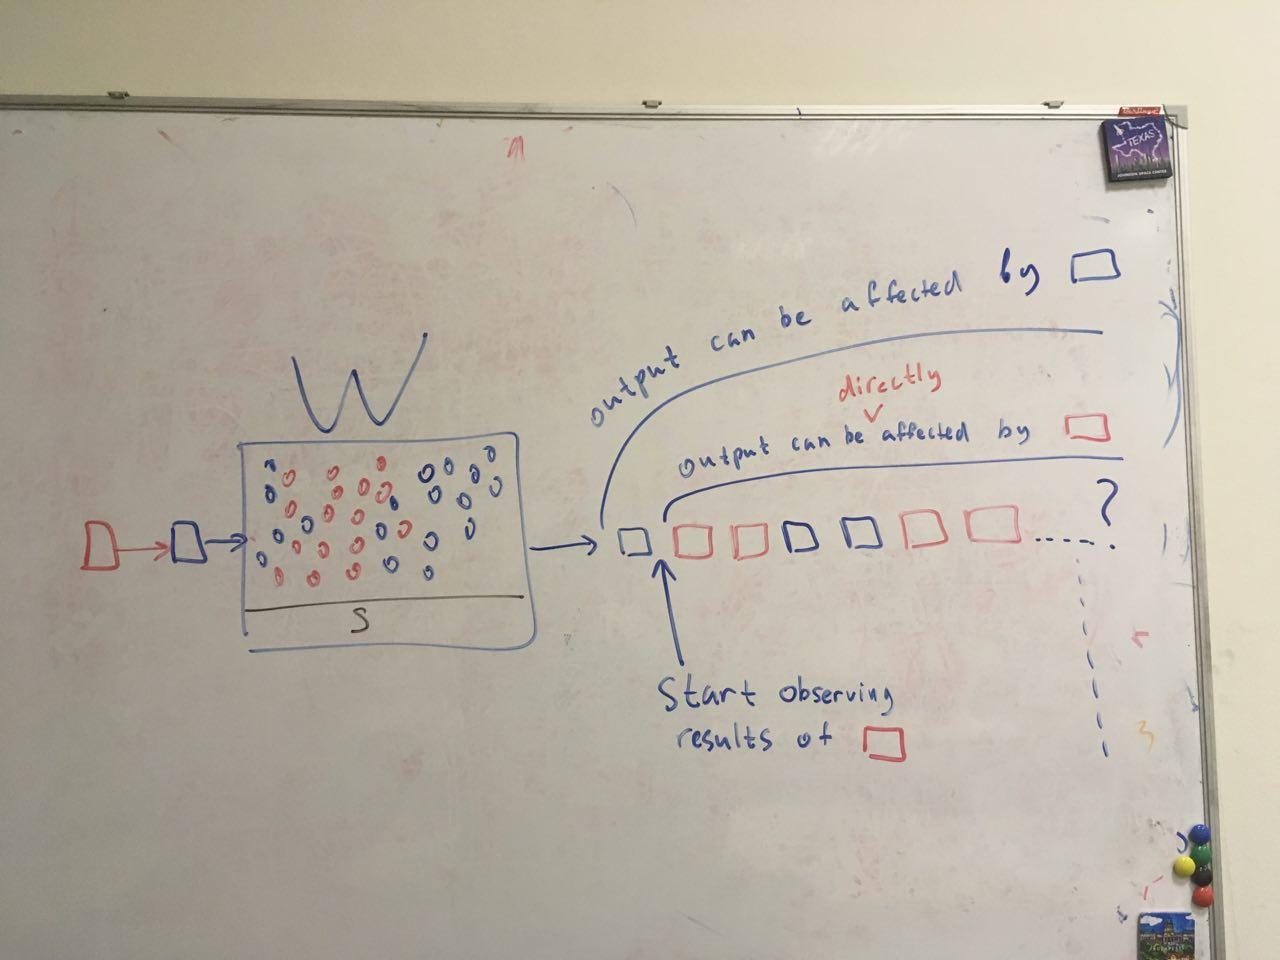
\includegraphics[width=0.48\textwidth]{pics/nullification}
%   \caption{The red and blue elements have entered the system. Since that time, it is unclear, when they stop directly affect output elements}
%   \label {nullification}
% \end{figure}

% \begin{definition}{Time quantization}
% $t$ is the time of input, output, and nullification:

% $t=\begin{cases}
% \tau_i:\exists{a_{\tau_i}}, \\
% \tau_o:\exists{b_{\tau_o}}, \\
% \theta_{a_\tau}:\forall{a_\tau}.
% \end{cases}$
% \end{definition}

% Time quantization allows us to consider only {\em observable} points in time. The time of input and output elements is obviously observed by any system. The mechanisms for tracking nullification vary slightly more. In Storm, a special agent called {\em Acker} is used. In Flink, nullification time is tracked using {\em low watermarks}. In Spark Streaming nullification time for each element in a micro-batch coincides with the time, when the micro-batch is fully processed.

% Let $x,a^{1},a^\infty$ be input elements with arbitrary arrival times. $\mathbb{B}_t$ are all output elements by the time $t$:

% $\mathbb{B}_t=\bigcup\limits_{i=1}^{t}{b_i}$

% Let $p(W_t,\mathbb{B}_t|x,a^{1}...a^\infty)$ be a probability to observe working set $W_t$ and output elements $B_t$ at the time $t$ if input elements are $x,a^{1},a^\infty$. Let us construct three sets:

% $X^0=(W_\infty,\mathbb{B}_\infty|p(W_\infty,\mathbb{B}_\infty|a^{1}...a^\infty)\neq{0})$

% $X^1=(W_{\theta_{x}},\mathbb{B}_{\theta_{x}}|p(W_{\theta_{x}},\mathbb{B}_{\theta_{x}}|x,a^{1}...a^\infty)\neq{0},\forall{i}:{a^i}\neq{x})$

% $X^{*}=(W_{\theta_{x}},\mathbb{B}_{\theta_{x}}|p(W_{\theta_{x}},\mathbb{B}_{\theta_{x}}|x,a^{1}...a^\infty)\neq{0},\\
% \exists{i}:{a^i={x}},\exists{y:y\in{W_{\theta_{x}}\setminus{S_{\theta_x}}}\cap{Cl(D)(a^i)}})$

% These sets model the {\em observable} output, current elements, and state of a stream processing engine. $X^0$ expresses the case, when element $x$ has not affected the system, so it is a forbidden behavior for at least once and exactly once guarantees. On the other hand, $X^{*}$ defines possible results, after $x$ has been nullified, but $a^i=x$ or its dependencies are in the system. Such behavior can cause inconsistencies in system state due to duplicates and should not be observed if the system provides for at most once or exactly-once. Using these modeled sets now we can define guarantees.

% \begin{definition}{At most once}
% guarantee is provided by a system iff $\forall{x,a^{1}...a^\infty}:X^{1}\cap{X^{*}}=\emptyset$
% \end{definition}

% \begin{definition}{At least once}
% guarantee is provided by a system iff $\forall{x,a^{1}...a^\infty}:X^{0}\cap{X^{1}}=\emptyset$
% \end{definition}

% \begin{definition}{Exactly once}
% guarantee is provided by a system iff $\forall{x,a^{1}...a^\infty}:X^{1}\cap{X^{*}}=\emptyset \wedge X^{0}\cap{X^{1}}=\emptyset$
% \end{definition}

% % Now streaming consistency guarantees are defined in terms of correspondences between input, output and the system state. Custom system or user-defined semantics are not considered in this model, e.g., if the system drops all input items, it also can be claimed as supporting exactly-once. Looking from another side, our model formally describes which properties are {\em exactly} supported by state-of-the-art stream processing systems, such as Flink, Storm, Spark Streaming, Samza, MillWheel, etc, so we can discuss its properties in unified terms.

% We defined streaming consistency guarantees in terms of the proposed model. This model is suitable for state-of-the-art stream processing systems, such as Flink, Storm, Spark Streaming, Samza, MillWheel, etc, so now we can discuss its properties in unified terms.

% \subsection{Implementation properties and notes}

% % In this section, we formally define some additional concepts and demonstrate a potential way to reduce latency overhead on consistency guarantees. We mainly consider exactly once, because it is the strongest guarantee, which is extremely valuable in practice.    

% \begin{definition}{System failures}
% are the time moments, when the system loses its working set. 
% \end{definition}

% Assume that the system fails at time $\tau_f$. The naive idea for recovering is to simply start processing from the very beginning, i.e., to set $W_{\tau_f+1}=\emptyset$ and to replay the whole input stream. However, storing and replaying the whole input stream is inefficient in terms of both memory and time consuming and can violate consistency guarantees.

% \begin{definition}{Snapshot}
% at time $\tau_s$ is persistently stored $P_{\tau_s}\subseteq{W_{\tau_s}}$ that is not lost even in case of failure.
% \end{definition}

% Snapshots allow a system to restart processing since defined points. One approach for taking snapshots is to save (or update) the whole $W_{\tau}$ on each $\tau$. In this case, there is no need to replay input elements, because the system can completely restore computations using only a snapshot. Google MillWheel uses this method for recovering. {\em Strong productions} mechanism allows MillWheel to preserve exactly-once guarantee for the price of persistent updates of $P_\tau=W_\tau$ on each $\tau$~\cite{Akidau:2013:MFS:2536222.2536229}.    

% Another approach is to take so-called {\em state snapshots}. This kind of snapshots is considered in practice only within the time quantization $t$. It assumes that $\forall{t_s}:P_{t_s}=S_{t_s}$ and requires replay of input element. Suppose, there is a state snapshot at time $t_s$ and a system fails at time $\tau_f>t_s$. In order to recover processing, system sets $W_{\tau_f+1}=P_{t_s}$ and requests for replay elements $a$ such that $\forall{y\in{Cl(D)(a)}}:y\notin{P_{t_s}}$. The idea of taking snapshots is illustrated in Figure~\ref{snapshotting}.

% \begin{definition}{Consistent state snapshot}
% $P^{c}_{t_s}=S_{t_s}$ at time $t_s$ is a snapshot such that $\forall{a}\in{Cl^{-1}(D)(P^{c}_{t_s})}:\exists{\theta_a}$.
% \end{definition}

% \begin{theorem}
% A system, that uses state snapshots for recovery, provides for at most once guarantee only if all state snapshots are consistent.  
% \end{theorem}

% Our notion of consistent state snapshot modifies the classical definition of {\em consistent distributed snapshot} proposed in~\cite{Chandy:1985:DSD:214451.214456} for the case where dependencies between messages exist and input element must be applied to state atomically with its inversed dependencies. This notion is natural for stream processing systems because as it was shown, it is directly connected with streaming consistency guarantees. 

% One popular method for taking consistent state snapshot is to artificially reproduce a moment $t_s$, when $\forall{a}\in{Cl^{-1}(D)(S_{t_s})}:\exists{\theta_a}$, and to save obtained $S_{t_s}$. Such approach is adopted in Apache Flink~\cite{Carbone:2017:SMA:3137765.3137777} and Apache Storm~\cite{apache:storm:state}. They achieve consistent state by injecting special elements called {\em checkpoints} into the input elements. Checkpoints go through the same network channels as ordinary elements and push all inverted dependencies of inputs through the system. Each operation in data flow prepares its snapshot independently at the moment of checkpoint arriving. Global snapshot is taken when checkpoint passes through the whole data flow. 

% Checkpoints cause latency overhead because they periodically block some inputs of an operation with multiple inputs. This behavior is known as {\em checkpoints alignment}. Consistent state snapshotting can be potentially relaxed if there is a mechanism to retrieve only a consistent part of each operation state at any moment in time. In this case, there is no need to technically reproduce a moment, when it is consistent, in order to obtain it.

% Another property that directly affects consistency guarantees is {\em determinism}. Let $a_1...a_\infty$ be ordered in time input elements.

% \begin{definition}{Data processing system is {\em deterministic}}
% if \\
% $\forall{t} \forall{n\geq1} \forall{a_1...a_n}\exists{\mathbb{B}_t={\{b_1...b_m\}}}:\sum\limits_{W_t} p(W_t,\mathbb{B}_t|a_1...a_n)=1$.
% \end{definition}

% \begin{theorem}
% A non-deterministic system provides for at most once guarantee only if $\forall{b_{t_o}}:\exists{P^{c}_{t_o}} \wedge \forall{a\in{Cl^{-1}(b_{t_o})}},\theta_a=t_o$.  
% \end{theorem}

% Hence, non-deterministic systems that use state snapshots must atomically output elements and take a consistent snapshot that contains their inverted dependencies in order to achieve exactly once. In practice, it means that the lower bound of latency in the worst case in such systems is the time between snapshotting together with the duration of taking a snapshot. There is a trade-off between latency and the frequency of taking snapshots because too frequent snapshotting can cause high extra load, while rare snapshots lead to high latency. We can observe such behavior in all stream processing systems that provide for exactly once and use state snapshots, e.g., in Flink atomicity between state snapshotting and elements releasing is preserved using the modification of 2PC protocol. On the other hand, if a system is deterministic, atomicity between output and snapshotting is not necessary, because in case of replay system releases exactly the same output, that can be somehow deduplicated.